\documentclass[10pt,a4paper]{article}
\usepackage[utf8]{inputenc}
\usepackage{spconf}
\usepackage{amsmath}
\usepackage{amsfonts}
\usepackage{amssymb}
\usepackage{lmodern}
\usepackage{graphicx}
\usepackage{float}
\usepackage{multicol}
\usepackage[xindy]{glossaries}
\usepackage[left=2cm,right=2cm,top=2cm,bottom=2cm]{geometry}

\usepackage[backend=biber]{biblatex}
\addbibresource{bibliography.bib}
\graphicspath{{graphics/}}

\twoauthors
  {R. Deliallisi}
  {
  	ETH Zürich, D-INFK\\
	{\small Rämistrasse 101, 8092 Zurich, SWITZERLAND}
  }
  {C. Trassoudaine\sthanks{Work performed while at ETH Zürich}}
  {
	  IMT Atlantique,\\
	  {\small 655 Avenue du Technopôle, 29280 Plouzané, FRANCE}\\
	  EURECOM, Data Science dpt.,\\
	  {\small 450 route des Chappes, 06410 Biot, FRANCE}
  }
  
\title{
	Robustness verifier heuritics for neural networks
}

%\usepackage{filecontents}
%\begin{filecontents}{bibliography.bib}
%@InProceedings{AI2,
%author = {T. Gehr M. Mirman D. Drachsler-Cohen P. Tsankov S. Chaudhuri M. Vechev},
%title = {AI2: Safety and Robustness Certification of Neural Networks with Abstract Interpretation},
%year = {2018},
%booktitle = {IEEE S\&P},
%}
%\end{filecontents}


\newacronym{nn}{NN}{neural-networks}
\newacronym{lp}{LP}{linear-programming}

\begin{document}

\maketitle

\section*{Introduction}

The purpose of this work is to prove formally the local-robustness of \gls{nn} by heuristically combining Box analysis and \gls{lp} solving. 
In this paper, we aim to present a time-efficient way of verifying \gls{nn} robustness large perturbations $\eta = \{\epsilon_0, ..., \epsilon_{n}\}$. We also make the simplification that the perturbation range is the same for each input neuron $n_{-1,i}$ such that the perturbed input $\hat{n}_{-1,i} = n_{-1,i} \pm \epsilon, \forall i \in \{1, ..., n\}$.

\section{Analysis techniques}
\subsection{Box analysis}

A very simple and fast approach to solve the \gls{nn} robustness problem is to use a polyhedra abstract domain as defined in [\footcite{AI2}]

\subsection{Linear programming}

\subsubsection{Range analysis}

\subsubsection{Robustness verification}

\section{Heuristics}

\begin{figure}[H]
\begin{center}
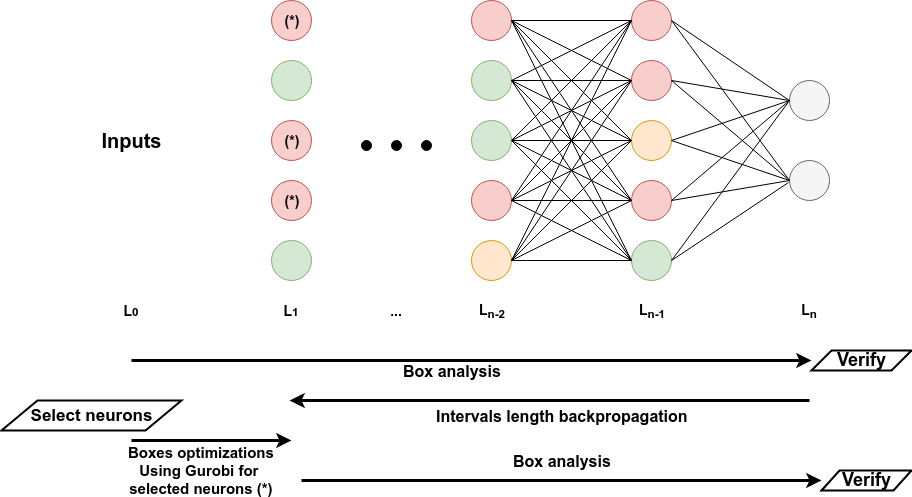
\includegraphics[width=6cm]{NN_lastlayer.png}
\caption{Last layers additionnal optimization}
\end{center}
\end{figure}

\section{Results}


\end{document}